\def\CC{{C\nolinebreak[4]\hspace{-.05em}\raisebox{.4ex}{\tiny\bf ++}}}
%
% 3 important ingredients for developing a simulation application like mirgecom which is designed to be a predictive simulation tool used in the design of scramjets.
%   [ Science into the code ]
%   - Physics (real device and model)
%      - Radiation
%      - Damage/degradation
%      - Material interface regression
%      - Coupling
%      - Mixture transport
%      - Turbulence
%   - Numerics (discretization, numerical methods)
%      - Model implementations
%      - ESDG (something else?! FV?)
%      - Hex elements
%      - Curvilinear Elements
%      - Mixed order or multi-volume with disparate orders

%   [ Science out of the code ]
%   - Performance (access to devices, utility, includes scientist interface); the efficacy with which the code can deliver meaningful discovery or data:
%      -- physics
%      -- numerics
%     - Computational scientist interface and workflow matter
%       -- MIRGE-Com (and deeper) API
%            -- driver continuity
%            -- bc refactor
%       -- PARSL
%       -- Data into and outof the code (visualization, (n-to-m) restart, analysis)
%       -- Development process matters here (also to our sponsors) [ reduce techdebt ]
%       -- Usage viscosity (bunch-o-outstanding developments)
%     - Reliability and confidence fits in here - and that means V&V
%       -- Development process matters here
%       - validation rest in the hands of the investigator(s)
%         -- but common UQ infrastructure can be facilitated
%             -- driver continuity, factor out init
%       - verification needs to be provided and facilitated
%             -- Testing infrastructure for sim developers (hpc platforms)
%                -- PARSL
%             -- MMS & symbolic infrastructure (performance of it too)
%             -- Verification, scoping, and testing at scale
%                 -- driver continuity
%                 -- testing infrastructure
%     - Delivering FLOPS on modern architectures (poised to provide more)
%       - impacts almost all other activities  [ Everyone ]
%       - Faster results [ Shelby, Nick ]
%       - Compile times (DAG splat) [ port Kaushik's trace call to arraycontext ]
%       - Helps Scoping runs, scientist workflow and development
%     - Understanding application performance in the lazy context [ Matthias ]
%       - built-in instrumentation (logpyle)
%       - Tagging [for info and functionality]
%       - Modeling and model verification
% - Understanding is then very important
%   - Experience with the tools
%      - Models
%      - Numerics
%      - Interface
%      - Performance
% - Separation of concerns
%
% 2 biggest things on fire for prediction
%     - prediction supporting performance? - performance
%     - can we do the prediction? - physics and numerics

\begin{frame}\frametitle{Outline}
% Legs of stool
\begin{center}
\mirgecom{}\\
https://github.com/illinois-ceesd/mirgecom
\end{center}
\vspace{15pt}
\begin{itemize}
\item Physics and modeling, numerics, performance 
  \begin{itemize}
%\item 3 pillars of prediction simulation
  \item Status
%\item Performance snapshot for \mirgecom{}
  \item Maybe some challenges
  \item Upcoming developments
  \end{itemize}
\item Y3 prediction developments, pain points
\item Focusing our efforts over the next few months
% heh :)
\end{itemize}
\end{frame}

\begin{frame}\frametitle{Performance}
\begin{center}
In general, performance is the reciprocal of the total time to solution (TTS). Where should we draw the line?\\
\vspace{40pt}
$\text{TTS} = T_\text{development} + T_\text{setup} + T_\text{simulation} + T_\text{analysis}$\\ 
\vspace{20pt}
$\text{Performance} = \frac{1}{\text{TTS}}$
\end{center}
\begin{tikzpicture}[remember picture, overlay]
\fill <2> [fill=white, opacity=0.7] (current page.south west) + (0.5,0.5) rectangle (12.5, 7.8);
  \node <2> [inner sep=0pt] at (current page.center) {
    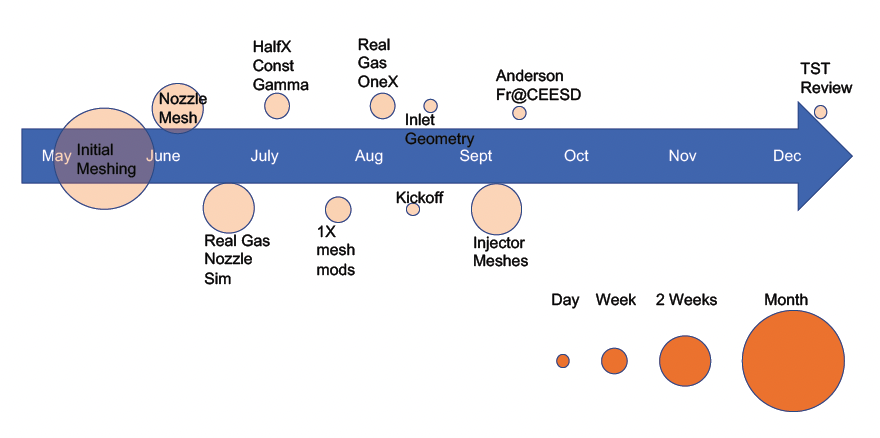
\includegraphics[width=.9\textwidth]{figures/workflow_timeline_1.png}
   };
\end{tikzpicture}
\end{frame}

\begin{frame}\frametitle{Performance}
\begin{center}
In general, performance is the reciprocal of the total time to solution (TTS). Where should we draw the line?\\
\vspace{40pt}
$\text{TTS} = T_\text{development} + T_\text{setup} + T_\text{simulation} + T_\text{analysis}$\\ 
\vspace{20pt}
$\text{Performance} = \frac{1}{\text{TTS}}$
\end{center}
\begin{tikzpicture}[remember picture, overlay]
\fill <2> [fill=white, opacity=0.7] (current page.south west) + (0.5,0.5) rectangle (12.5, 7.8);
  \node <2> [inner sep=0pt] at (current page.center) {
    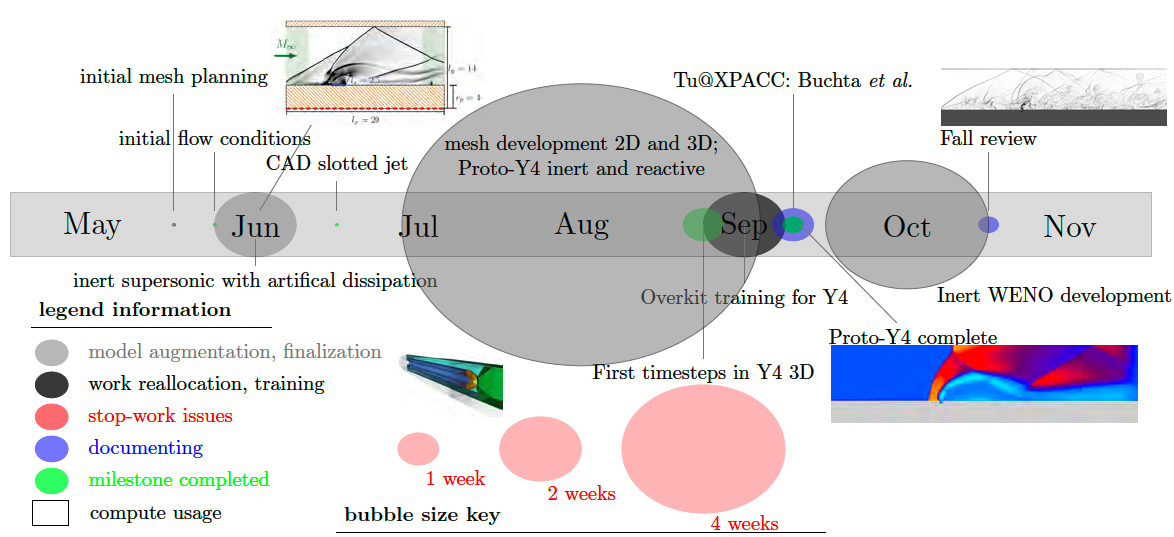
\includegraphics[width=.9\textwidth]{figures/workflow_timeline_2.png}
   };
\end{tikzpicture}
\end{frame}

\begin{frame}\frametitle{Performance}
\begin{center}
In general, performance is the reciprocal of the total time to solution (TTS). Where should we draw the line?\\
\vspace{40pt}
$\text{TTS} = T_\text{development} + T_\text{setup} + T_\text{simulation} + T_\text{analysis}$\\ 
\vspace{20pt}
$\text{Performance} = \frac{1}{\text{TTS}}$
\end{center}
\end{frame}

\begin{frame}\frametitle{Physics and Modeling}
\begin{center}
Current status
\end{center}
\begin{multicols}{2}
\begin{itemize}
\item Compressible Navier-Stokes
\item Nonlinear diffusion
\item Mixtures and combustion (simple transport)
\item AV/Shock capturing (art. physical visc)
\item Fluid no/slip, adiabatic/isothermal, in/outflow
\item Rigid wall/sample; heat eqn, ox diffusion, mass loss
\item Fluid/wall thermal coupling
\end{itemize}
\end{multicols}
\begin{center}
Development on the horizon
\end{center}
\begin{multicols}{2}
\begin{itemize}
\item Fluid/wall coupling updates (phenolics)
\item Mixture transport properties
\item Radiation model
\item Turbulence model
\item Degradation: fluid/wall interface regression
\end{itemize}
\end{multicols}
\end{frame}

\begin{frame}\frametitle{Numerics and Discretization}
\begin{center}
Current status
\end{center}
\begin{multicols}{2}
\begin{itemize}
\item Discontinuous Galerkin (DG)
\item Parallel, multi-volume, high-order tetrahedral meshes
\item Spectral filtering
\item Overintegration
\end{itemize}
\end{multicols}
\begin{center}
Development on the horizon
\end{center}
\begin{multicols}{2}
\begin{itemize}
\item New model implementations
\item ESDG \prj{\tiny}{Zirui Wang, T.~Gibson}
%\item Slope limiters
\item Quad/Hex support \prj{\tiny}{Addison Alvey-Blanco}
\item Mixed order or multi-volume with disparate orders
\item Curvilinear elements
\item Whole new method!? FV?
\end{itemize}
\end{multicols}
\end{frame}

\begin{frame}\frametitle{Performance}
\begin{center}
Current status
\end{center}
\begin{multicols}{2}
\begin{itemize}
\item Prediction-enabling performance (new this cycle)
\begin{itemize}
\item OOM: SVM/Unified memory
\item Dag Splat: 1D partitioning
\item Mem growth: Garbage collection
\end{itemize}
\item Scaling as expected (mostly)
%\item Absolute performance could be better
%\item Recent focus: memory growth
\item Small problems are expensive
\end{itemize}
\end{multicols}
\begin{center}
Grid Scaling\\
%\end{center}
%\begin{center}
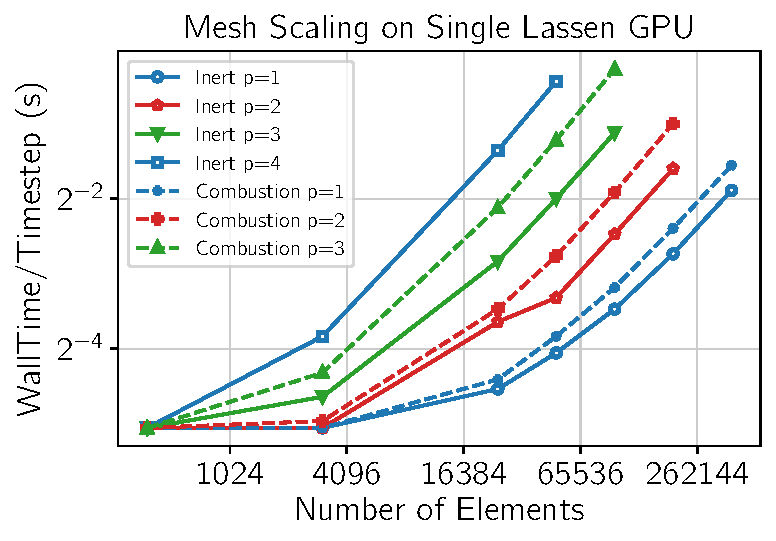
\includegraphics[width=.48\textwidth]{figures/mtc2/combozzle_gridscale.pdf}
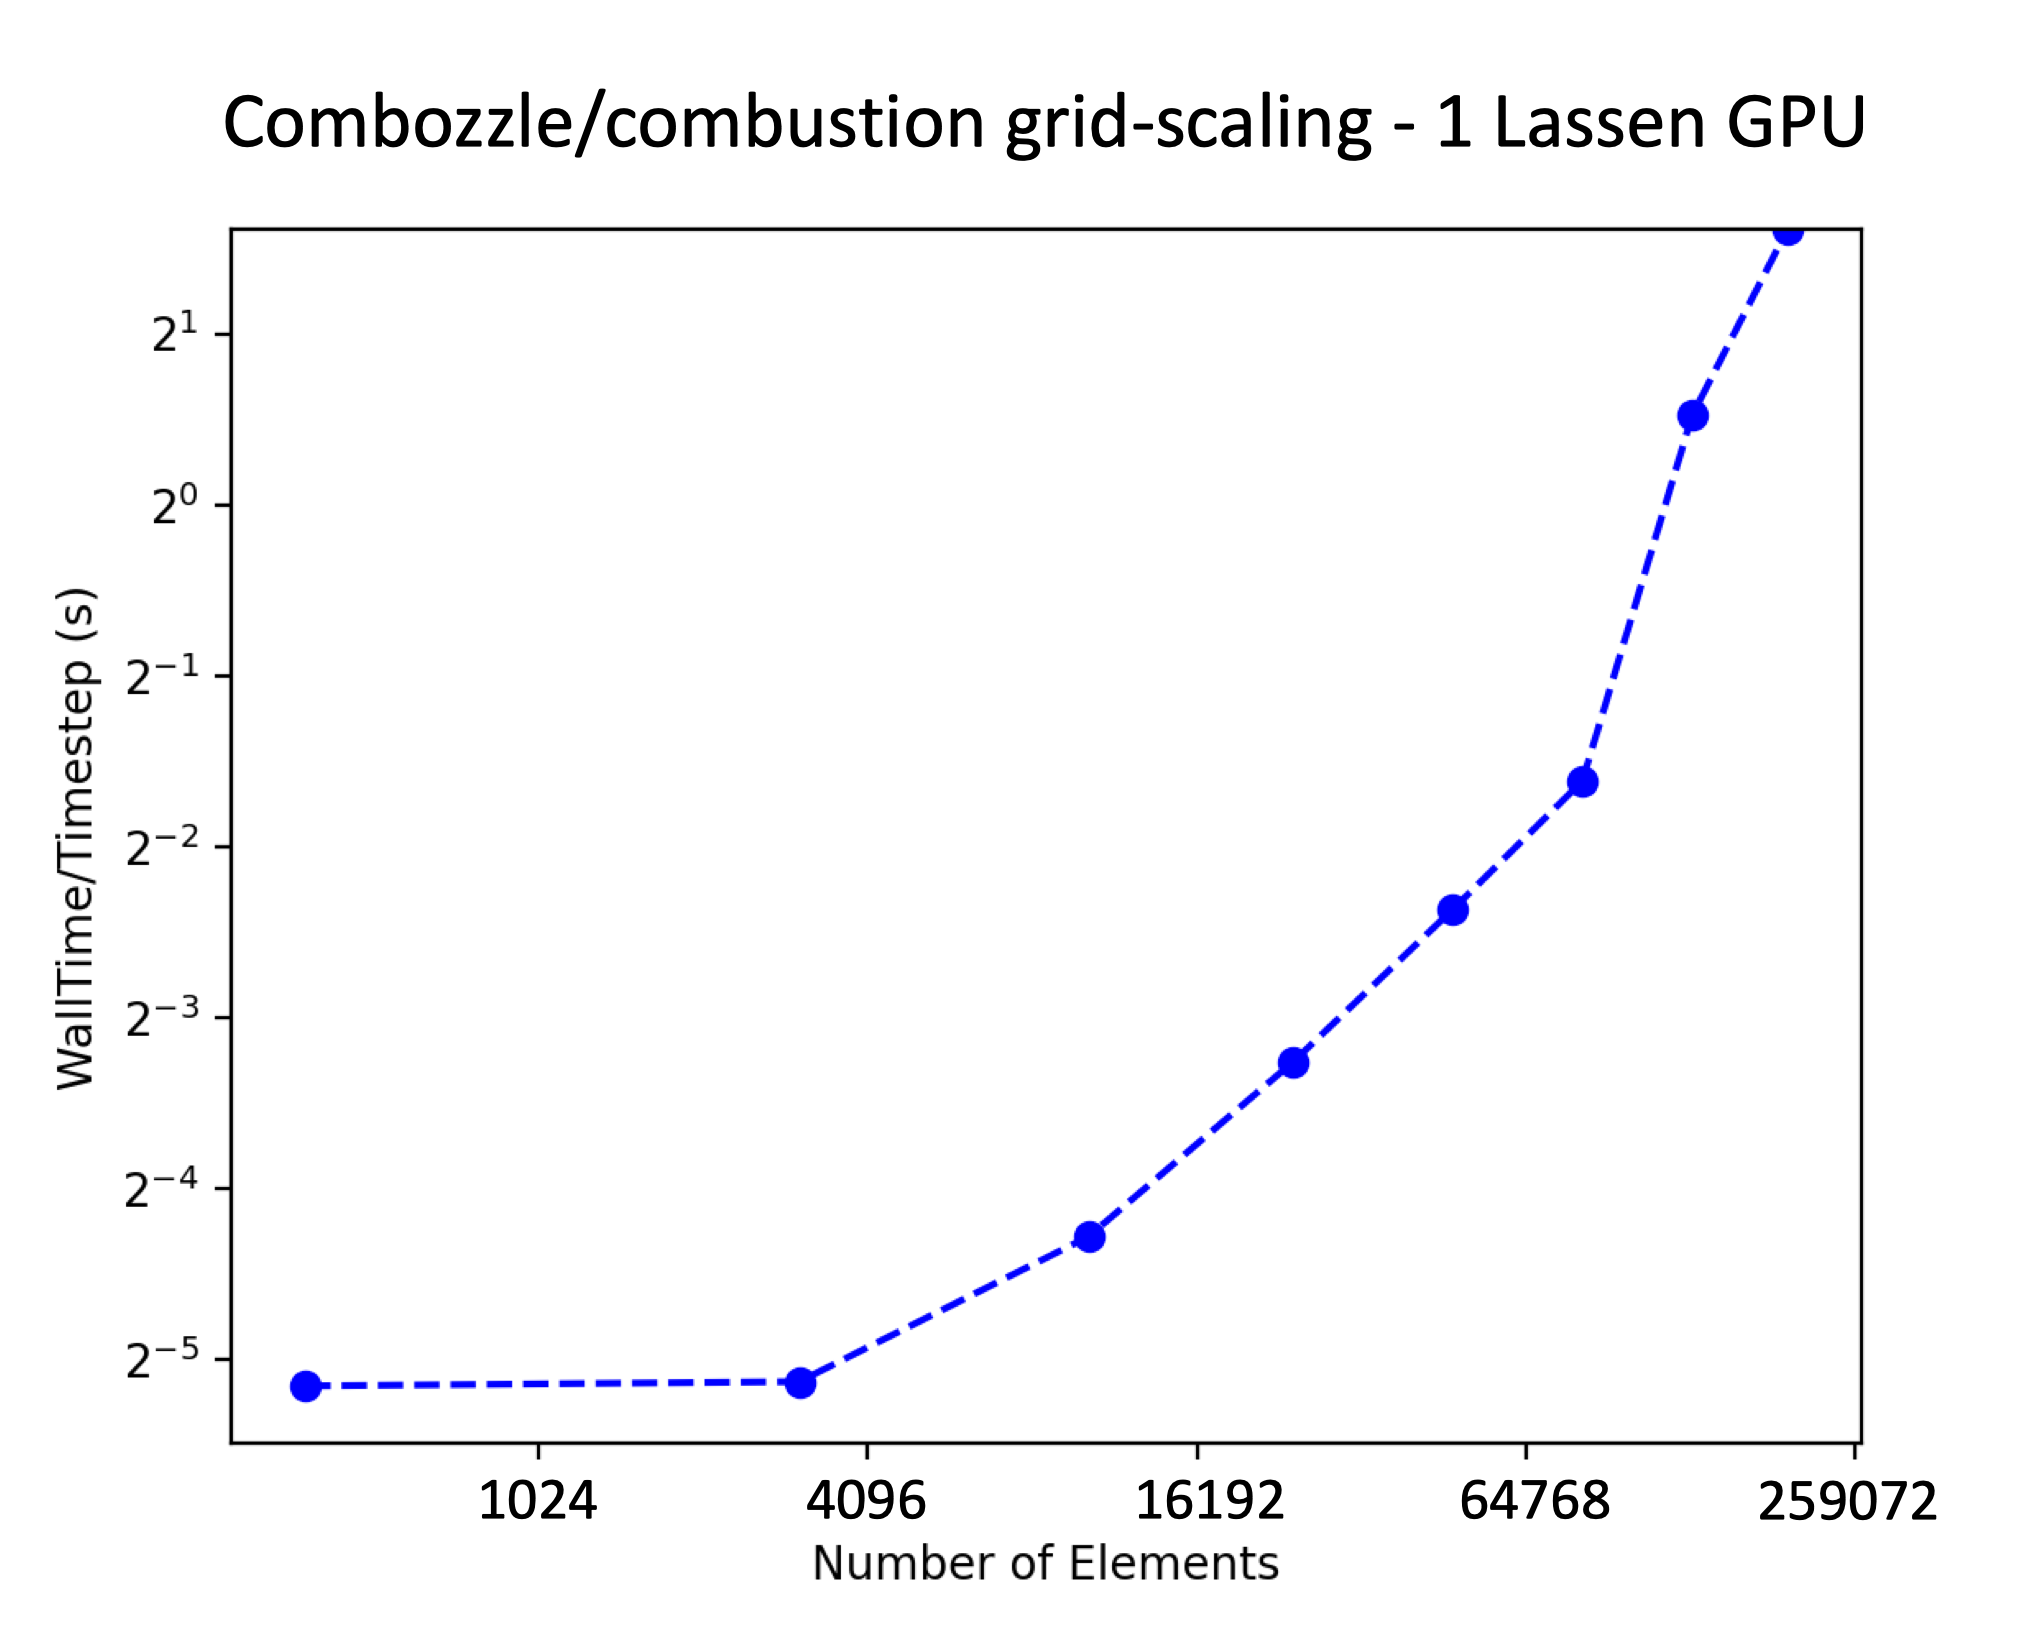
\includegraphics[width=.48\textwidth]{figures/comboz_gridscale_svm.png}
\end{center}
\end{frame}

\begin{frame}\frametitle{Performance}
\begin{center}
Current status
\end{center}
\begin{multicols}{2}
\begin{itemize}
\item Prediction-enabling performance (new this cycle)
\begin{itemize}
\item OOM: SVM/Unified memory
\item Dag Splat: 1D partitioning
\item Mem growth: Garbage collection
\end{itemize}
\item Scaling as expected (mostly)
%\item Absolute performance could be better
%\item Recent focus: memory growth
\item Small problems are expensive
\end{itemize}
\end{multicols}
\begin{center}
Weak Scaling (fixed work per GPU)\\
\end{center}
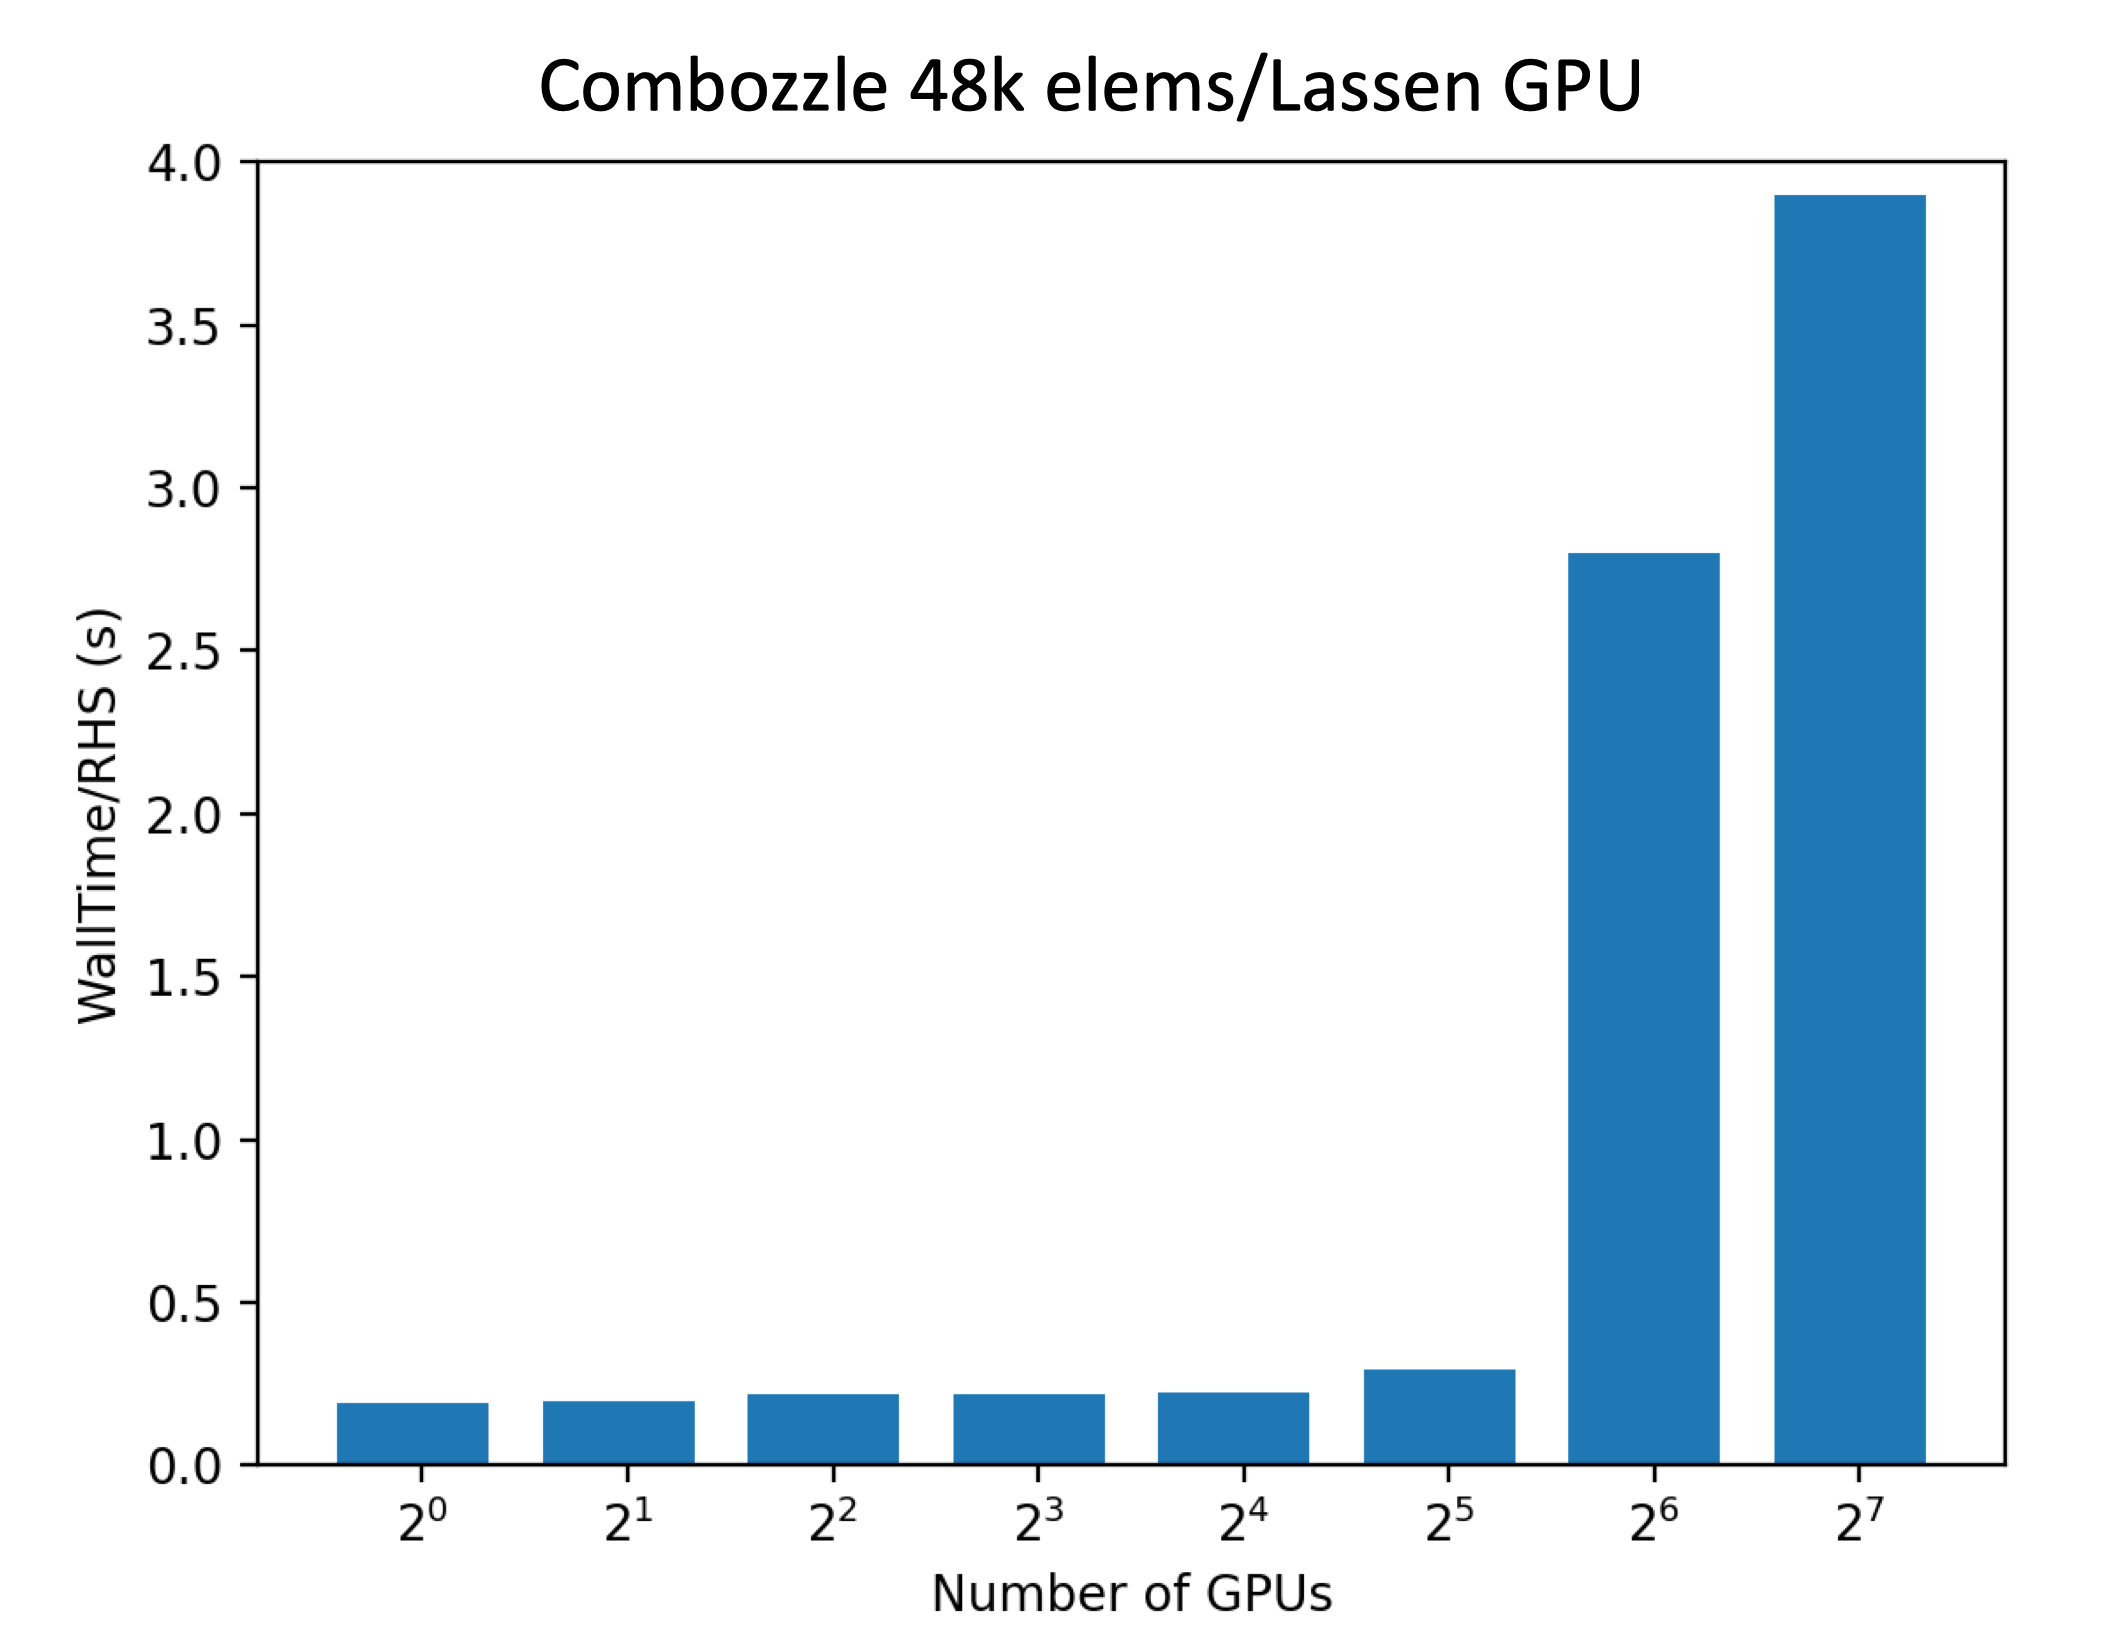
\includegraphics[width=.48\textwidth]{figures/combozzle_weak_bad_partitioning.png}
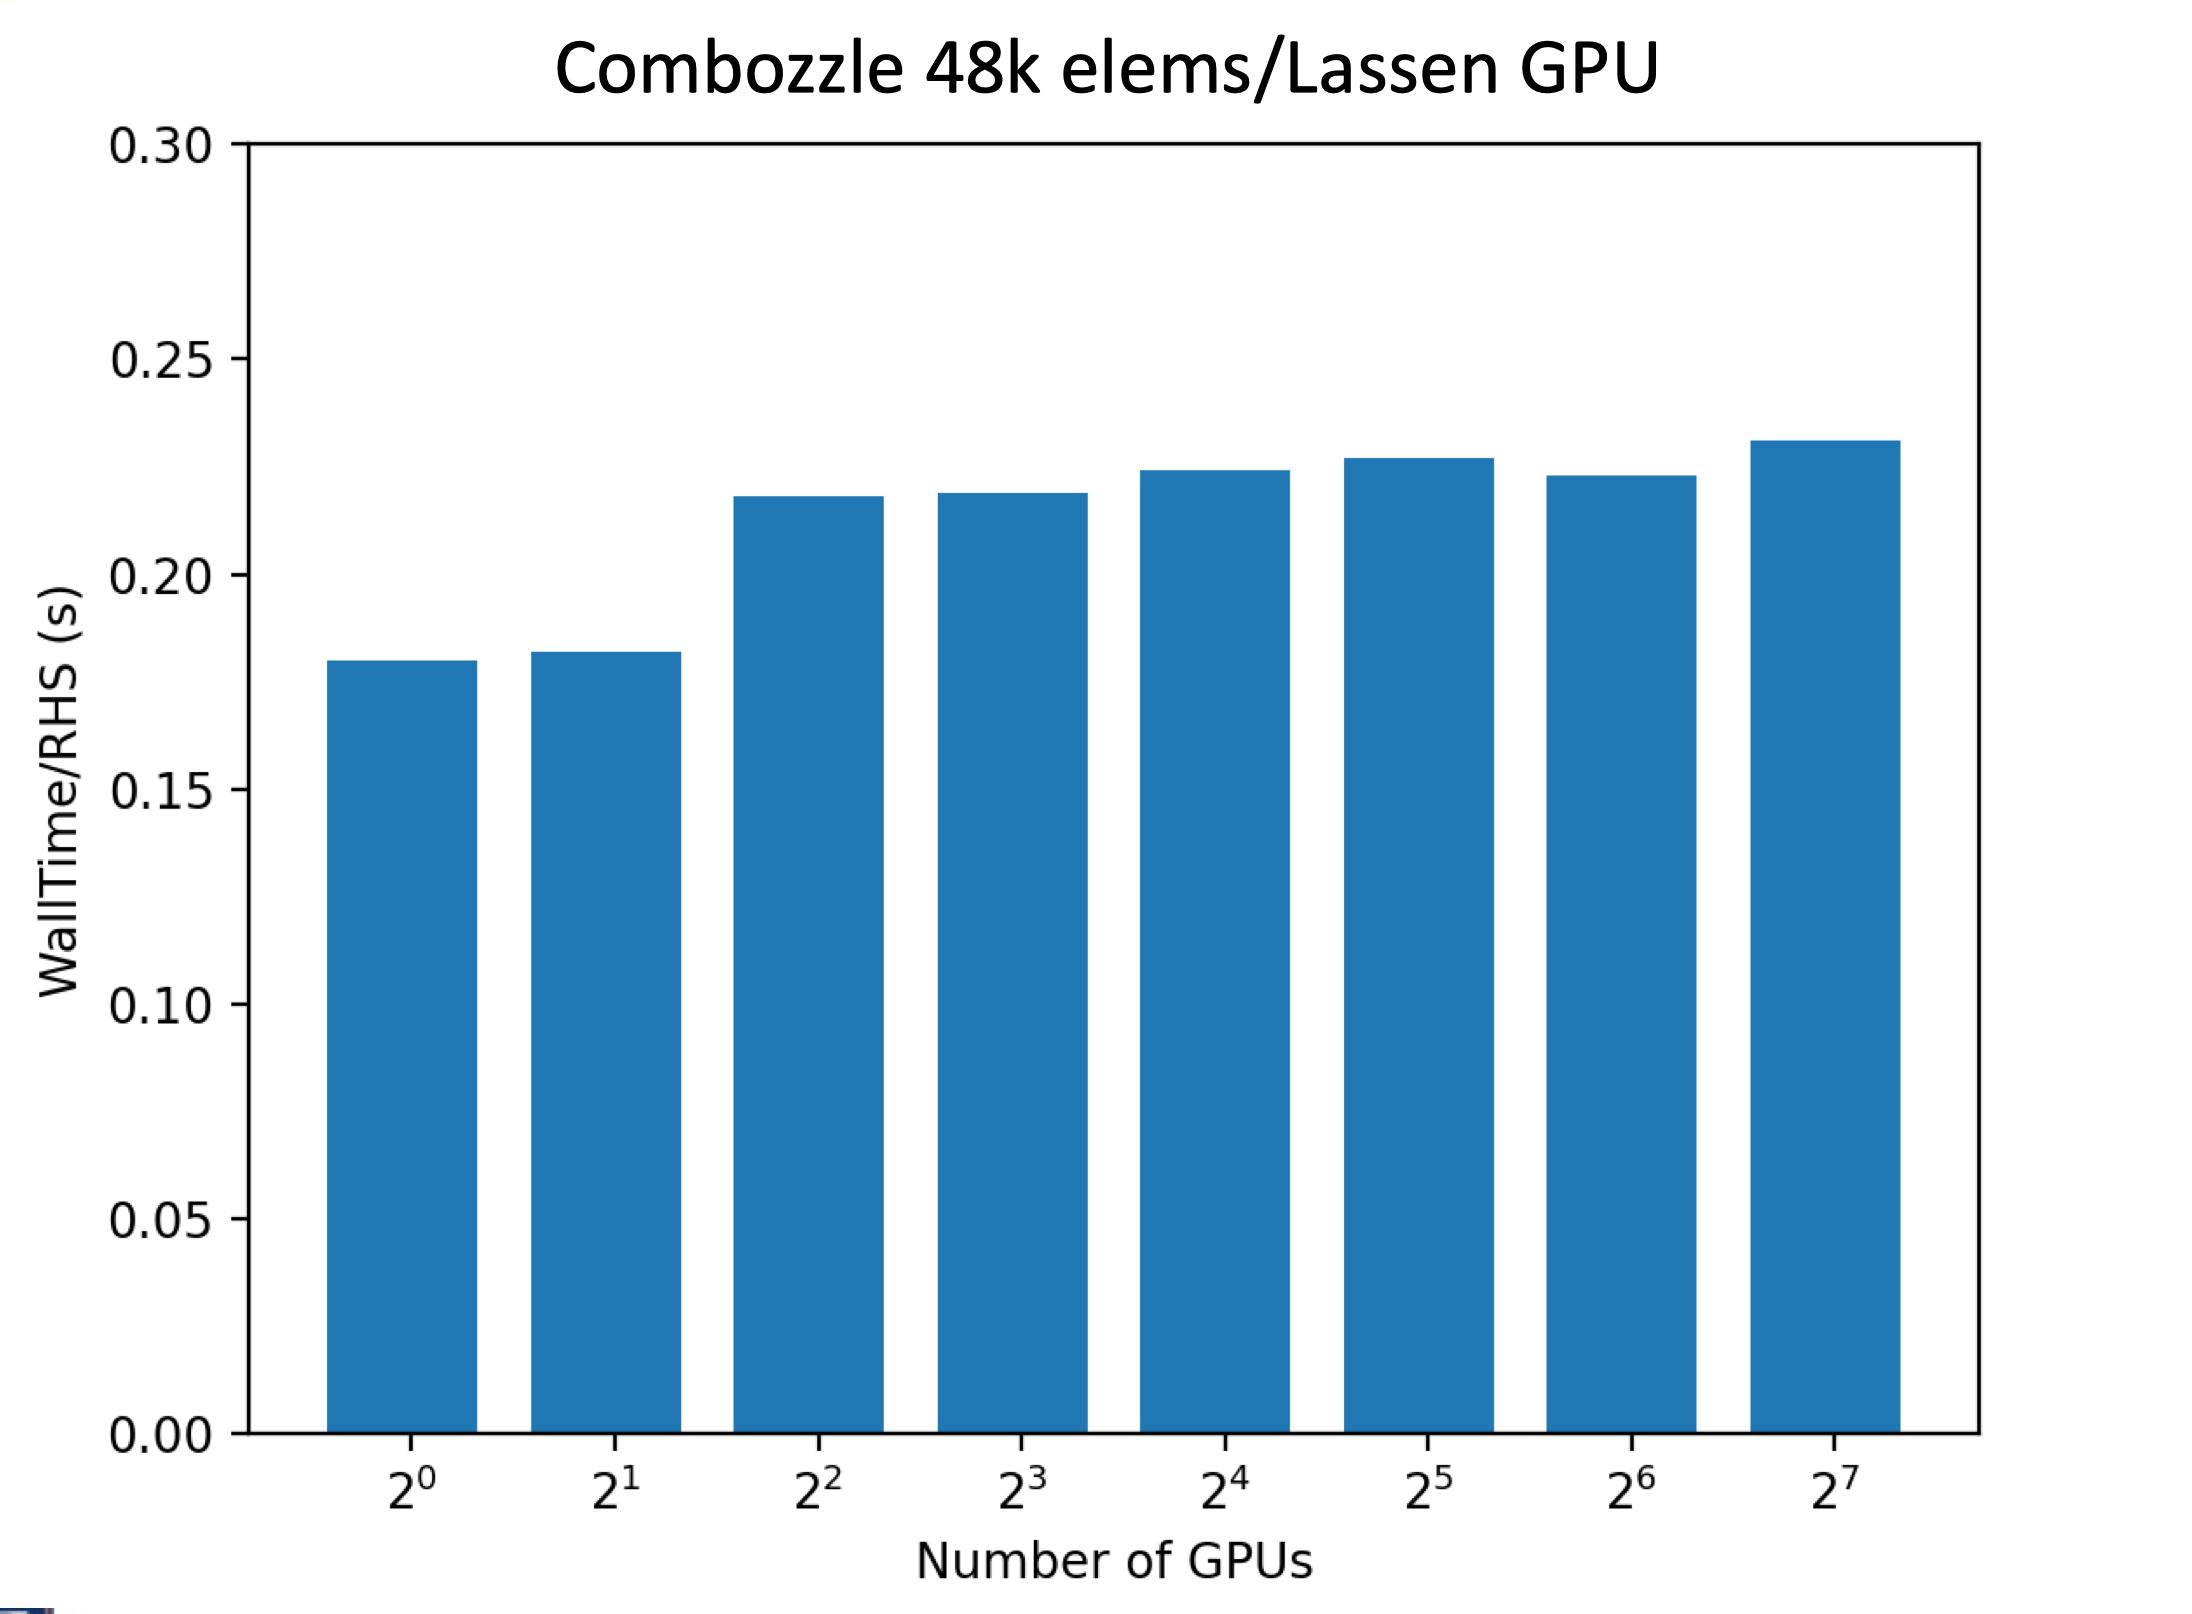
\includegraphics[width=.48\textwidth]{figures/combozzle_weak_sliced_partitioning.png}
\end{frame}

\begin{frame}\frametitle{Performance}
\begin{center}
Current status
\end{center}
\begin{multicols}{2}
\begin{itemize}
\item Prediction-enabling performance (new this cycle)
\begin{itemize}
\item OOM: SVM/Unified memory
\item Dag Splat: 1D partitioning
\item Mem growth: Garbage collection
\end{itemize}
\end{itemize}
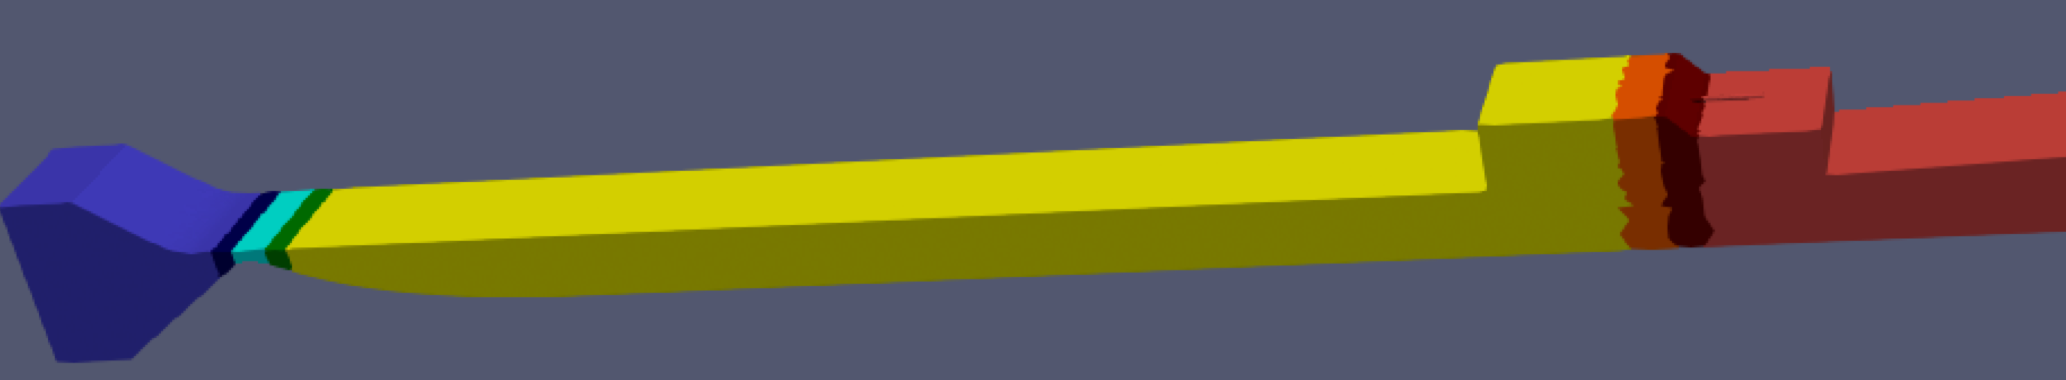
\includegraphics[width=.48\textwidth]{figures/1dpart_bal.png}
\columnbreak
\begin{itemize}
\item Scaling as expected (mostly)
%\item Absolute performance could be better
%\item Recent focus: memory growth
\item Small problems are expensive
\end{itemize}
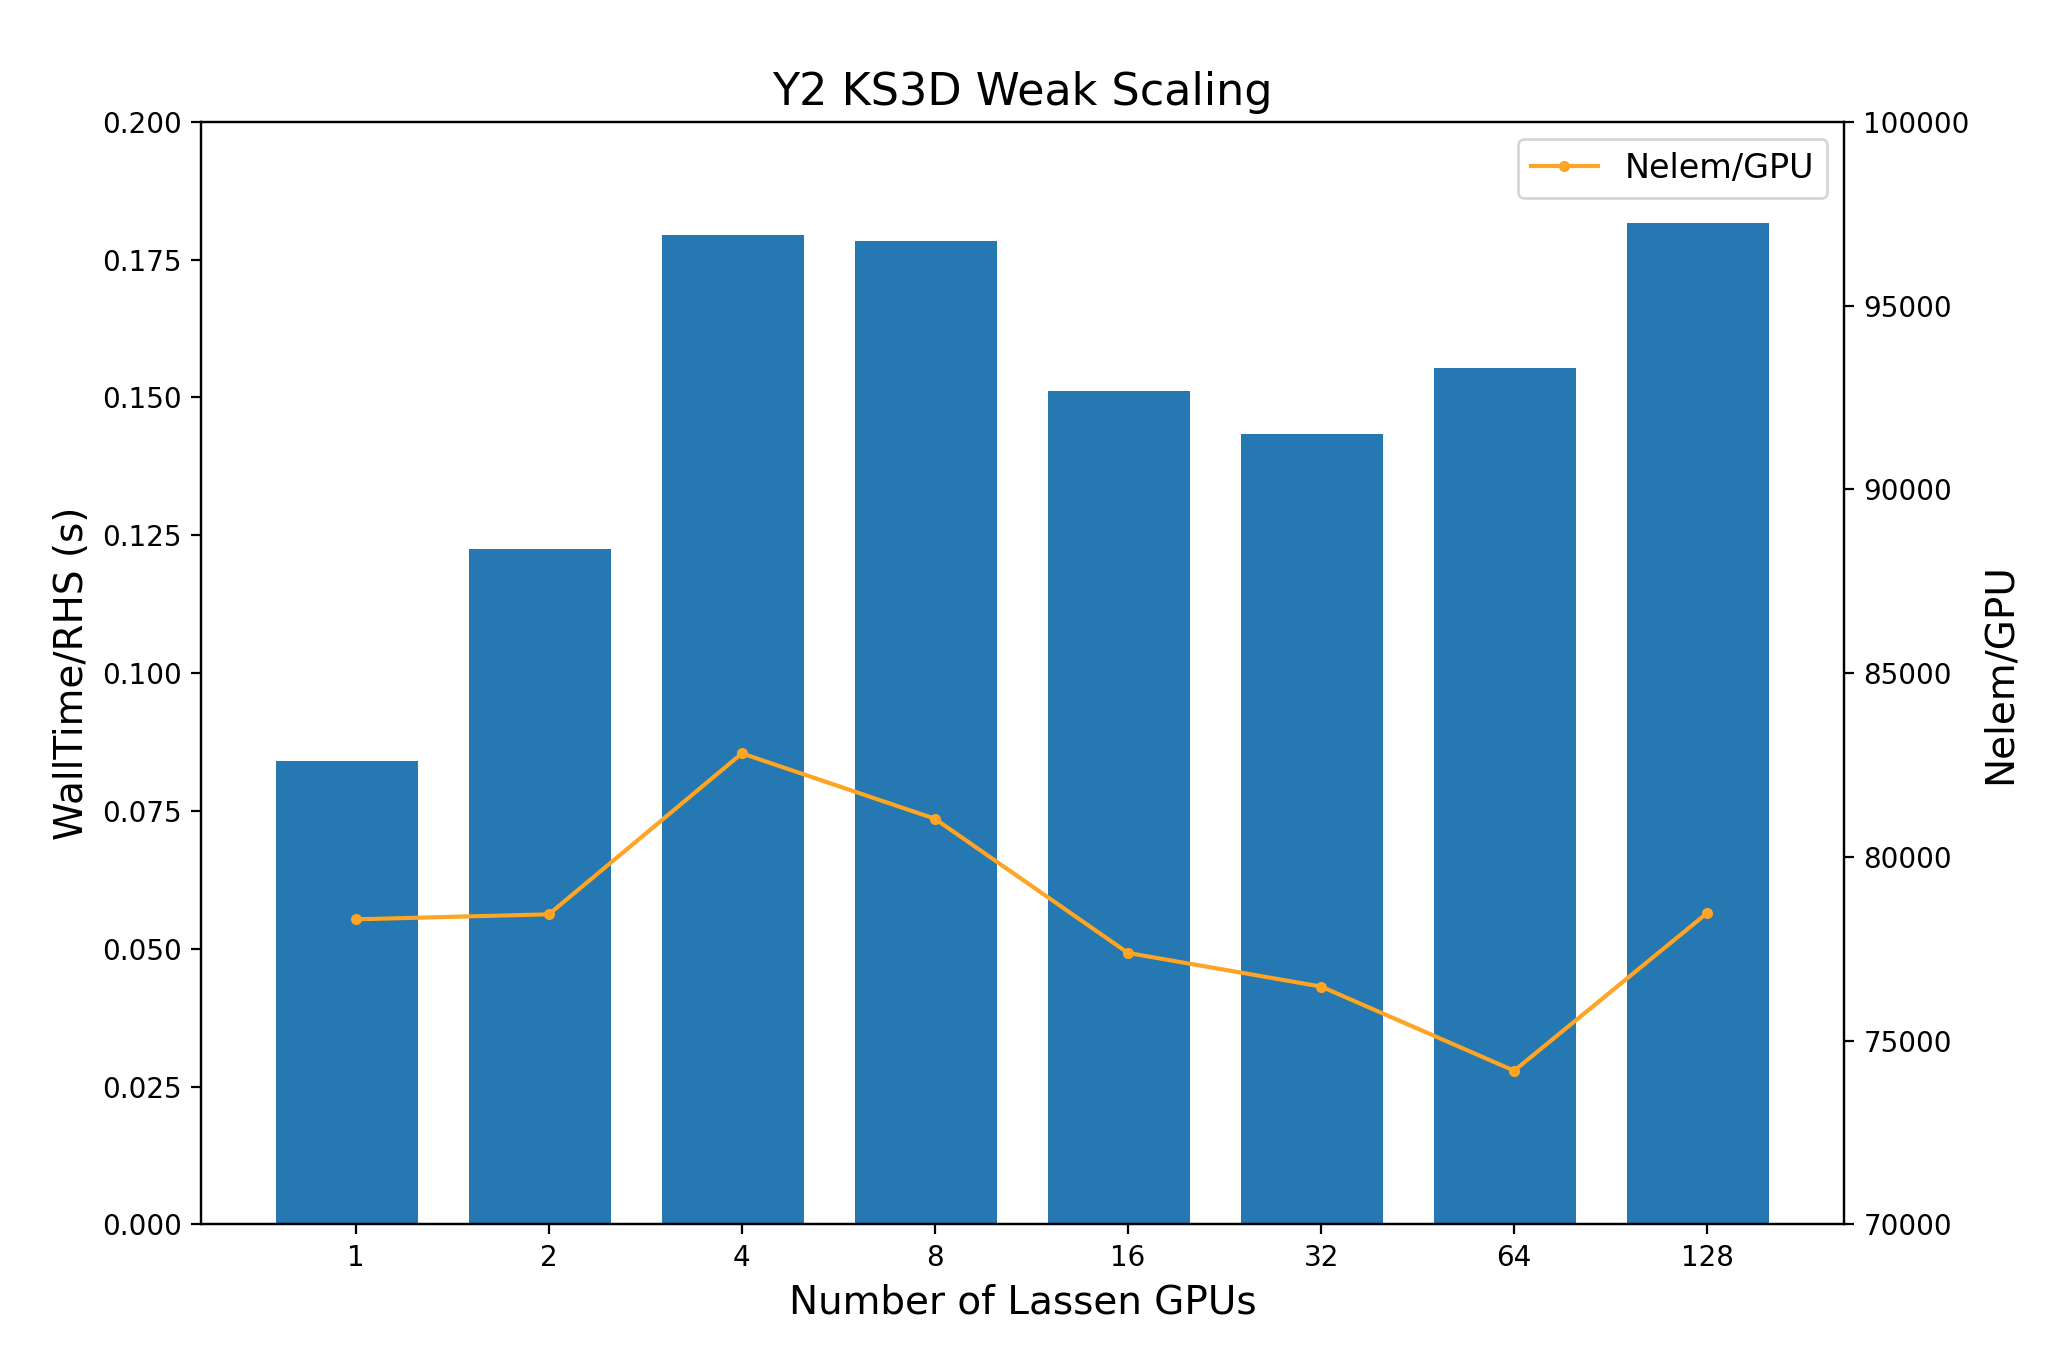
\includegraphics[width=.48\textwidth]{figures/y2ks3d_weak.png}
\end{multicols}
%\begin{center}
%Weak Scaling Prediction\\
%\end{center}
\end{frame}

\begin{frame}\frametitle{Performance Monitoring on Lassen}
\begin{center}
https://github.com/illinois-ceesd/timing\\
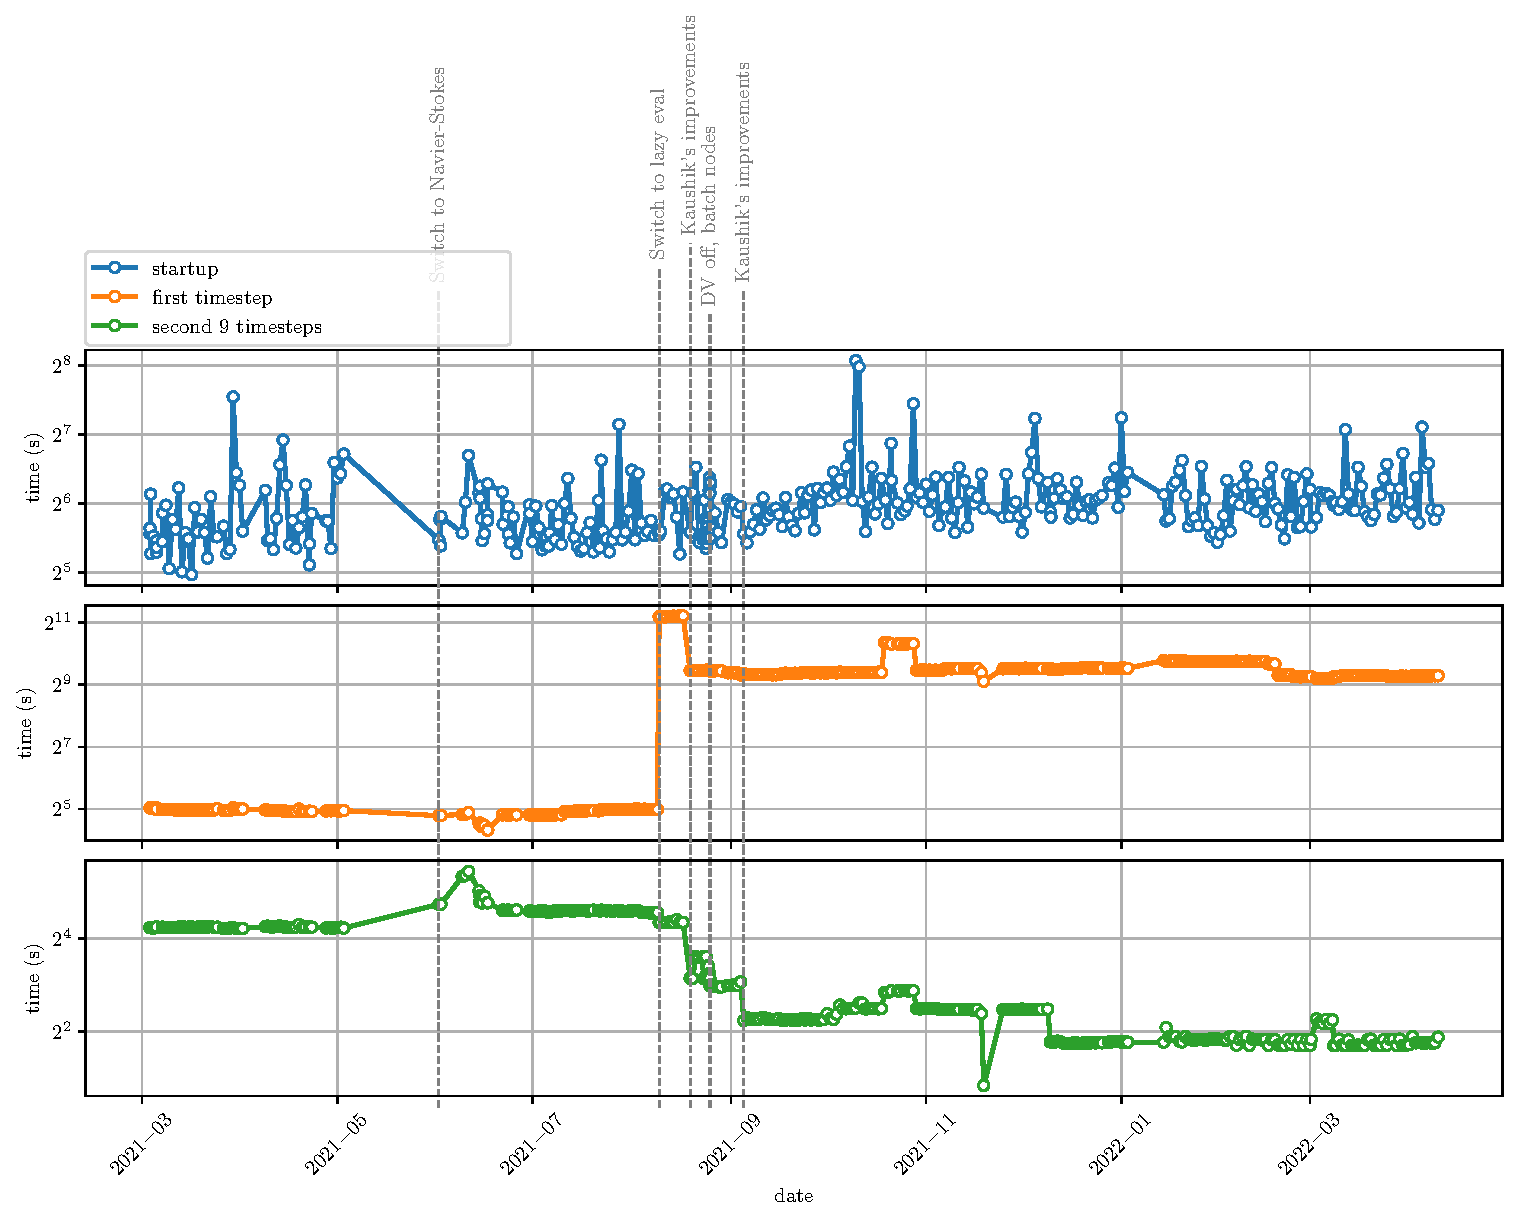
\includegraphics[width=.75\textwidth]{figures/mtc2/nozzle-lazy-full.pdf}
\end{center}
\end{frame}

\begin{frame}\frametitle{Performance Monitoring on Lassen}
\begin{center}
https://github.com/illinois-ceesd/timing
\end{center}
\begin{multicols}{2}
\begin{itemize}
\item Data on several cases collected nightly
\item Intended to track performance vs. code/features
\item New this cycle:
\begin{itemize}
\item Multi-case/comparitive plotting
\item Tracking parallel cases
\end{itemize}
\end{itemize}
\end{multicols}
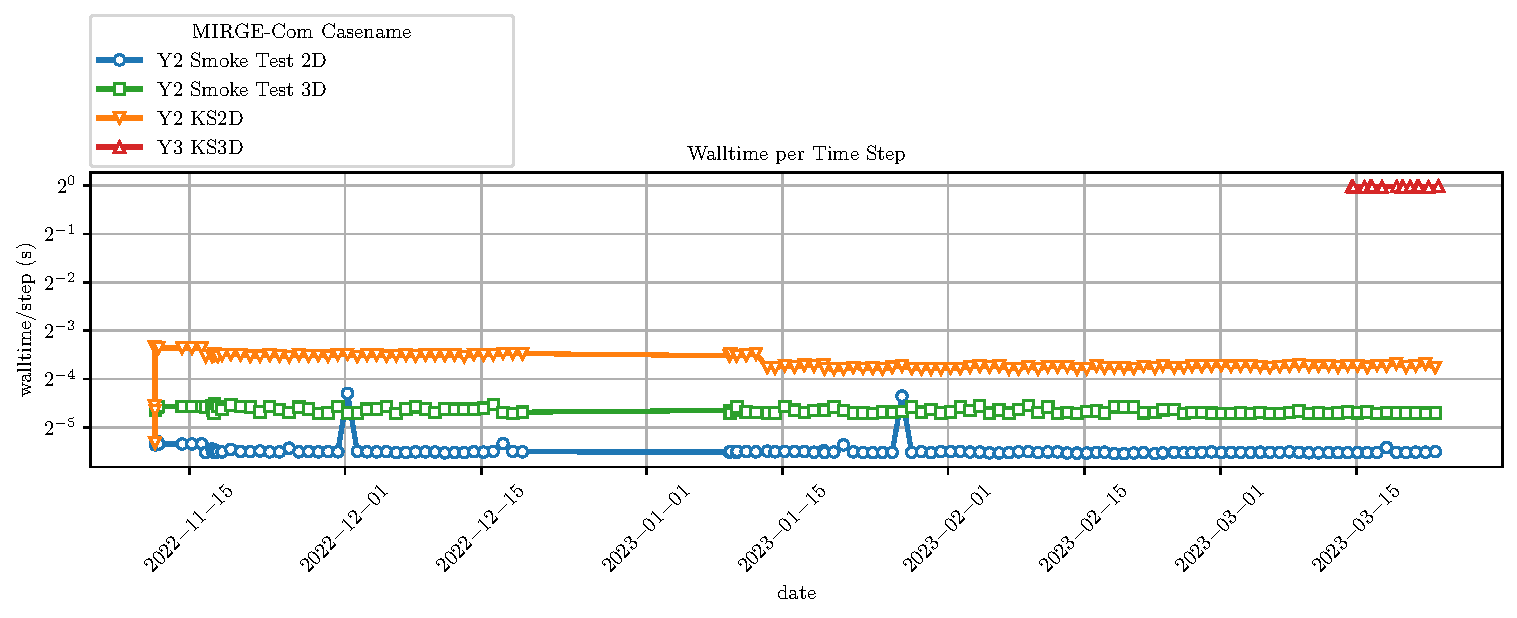
\includegraphics[width=\textwidth]{figures/multicase_step.pdf}
\end{frame}

\begin{frame}\frametitle{Performance Monitoring on Lassen}
\begin{center}
https://github.com/illinois-ceesd/timing
\end{center}
\begin{multicols}{2}
\begin{itemize}
\item Data on several cases collected nightly
\item Intended to track performance vs. code/features
\item New this cycle:
\begin{itemize}
\item Multi-case/comparitive plotting
\item Tracking parallel cases
\end{itemize}
\end{itemize}
\end{multicols}
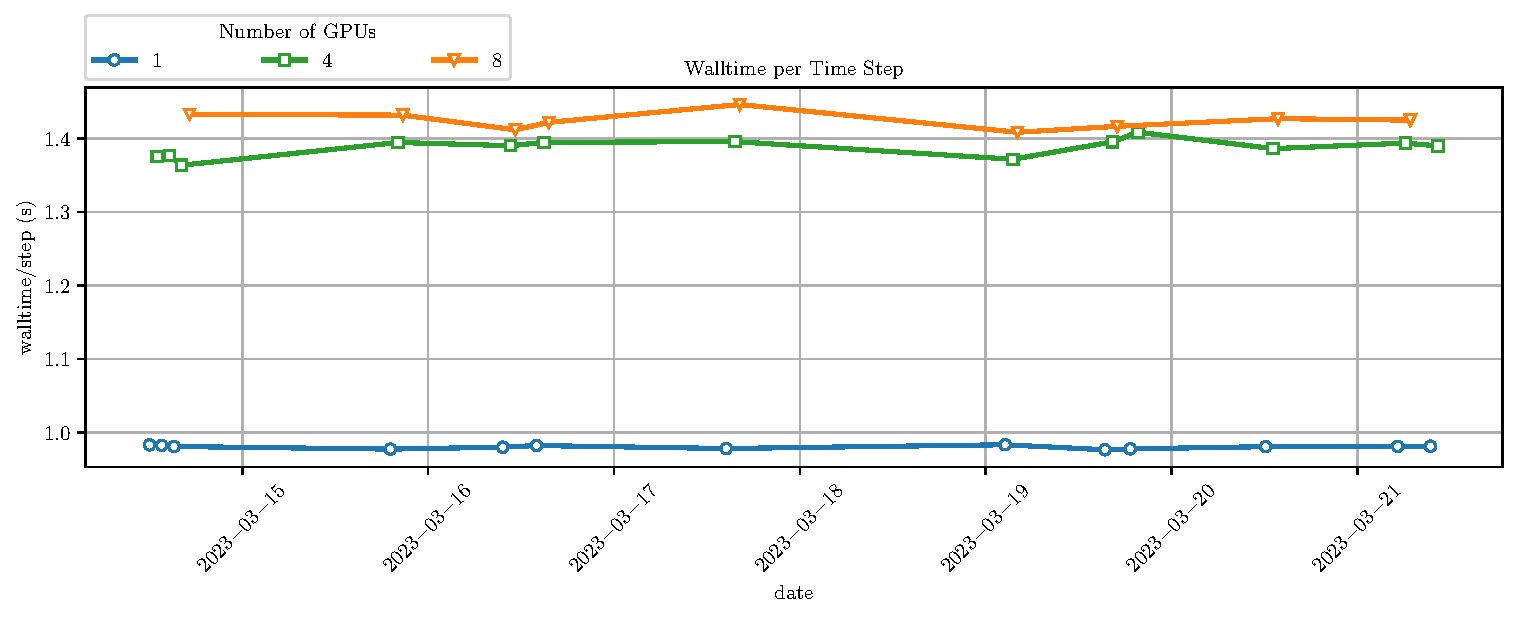
\includegraphics[width=\textwidth]{figures/prediction-scaling-tracking.pdf}
\end{frame}

\begin{frame}\frametitle{Performance-Driven Developments}
\begin{multicols}{2}
\begin{itemize}
\item Some pain-points
\begin{itemize}
%\item Lack of understanding \mirgecom{} performance
\item Code-to-kernel correspondence
\item Memory footprint is big
\item Scoping runs are a trudge (long turn-around)
\end{itemize}
\item Upcoming developments
\begin{itemize}
\item Performance model
\item PARSL \prj{\tiny}{D.~Friedel}
\item Auto-tuning \prj{\tiny}{Nick Christensen}
\item Node-aware communicators \prj{\tiny}{Shelby Lockhart}
\item DAG/compile time improvements \prj{\tiny}{Kaushik Kulkarni, M.~Diener}
\item Instrumentation (Mem \& Tags) \prj{\tiny}{Kaushik Kulkarni, M.~Diener}
\item \sout{DAG Splat} \prj{\tiny}{Kaushik Kulkarni}
\end{itemize}
\end{itemize}
\columnbreak
\end{multicols}
\vspace{-20pt}
\begin{center}
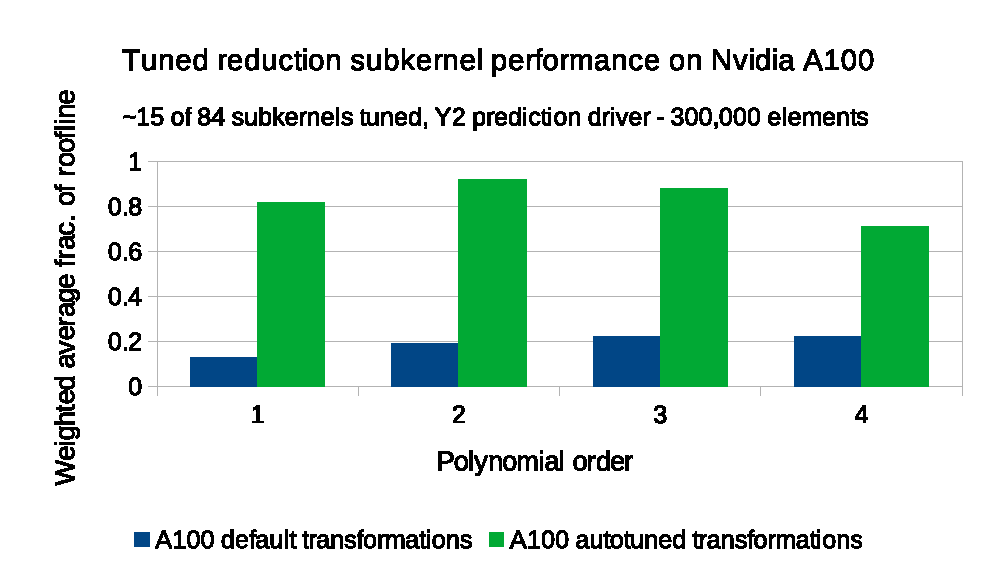
\includegraphics[width=.5\textwidth]{figures/Nvidia-A100-performance.eps}
\end{center}
\end{frame}

% - PLANS CHANGE
\begin{frame}\frametitle{Developments for Y3 Prediction}
\begin{center}
Y3 Driver\\
https://github.com/illinois-ceesd/drivers\_y3-prediction
\end{center}
\begin{multicols}{2}
\begin{itemize}
\item Kitchen sink (KS) feature set
  \begin{itemize}
  \item Coupled CNS + Wall/heat
  \item Ethylene mixture, reaction sources, species limiting, power-law transport
  \item Wall degradation, oxygen diffusion, reactive/porous mat.
  \item Artificial physical viscosity, and sponge
  \item OFF: Mixture transport, spectral filtering on RHS
  \end{itemize}
\item Meshes: 2D/3D updated geom, 2 test sects., shallower cavity
\item Sims: 3D coupled (6M,p=4 256 GPUs), and smaller
\item Scalability scripting and inputs (@add-scalability)
\end{itemize}
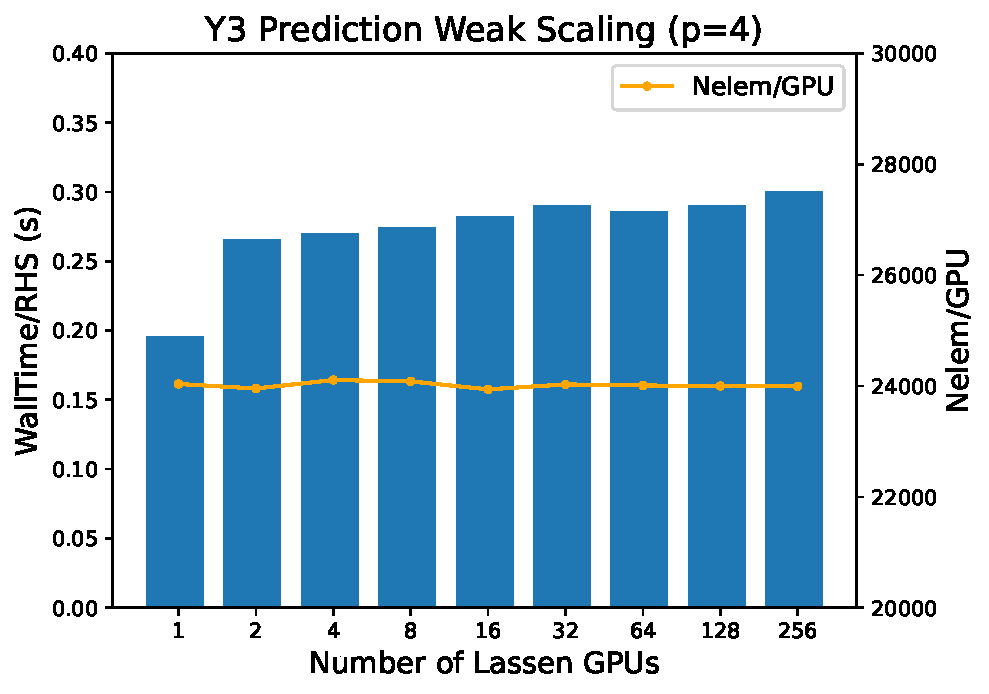
\includegraphics[width=.48\textwidth]{figures/y3-prediction_weak_scaling.pdf}
\end{multicols}
\end{frame}

\begin{frame}\frametitle{Path to Y3 Prediction}
\begin{multicols}{2}
\begin{itemize}
\item Physics and modeling: Radiation \& Phenolics (mild gap)
\item Numerics and discretization
  \begin{itemize}
  \item Mesh modifications (upstream injector, possible refinement)
  \item Maybe (gaps suspected):
    \begin{itemize}
    \item Higher order mesh + filtering (likely!)
    \item New AV
    % \item Slope limiters
    \item Multi-order meshes/volumes
    \item ESDG? \prj{\tiny}{Zirui Wang}
    \item Stop gap: High viscosity, maybe reduced physics
    \end{itemize}
  \end{itemize}
\columnbreak
\item Performance - closing gaps
  \begin{itemize}
  \item Cost per step (inert, comb): (.5, 1.4)s
  \item Sim time: 1ms inert, 6e-4 w/comb
  \item Estimated DT: .5ns
  \item 12d inert, 19d comb
  \item Any improvements welcomed
  \end{itemize}
\end{itemize}
\end{multicols}
\end{frame}

\begin{frame}\frametitle{Path to Y3 Prediction}
\begin{center}
\item Preparing for prediction runs
\end{center}
\begin{multicols}{2}
\begin{itemize}
\item 3M(ish) 3D p=3 elems 
\item Potentially serious issues: Shock/boundary, fluid/material
\item Investigating higher order, with filtering, high visc
\item Many scoping, physics-targeted, and debugging runs
\end{itemize}
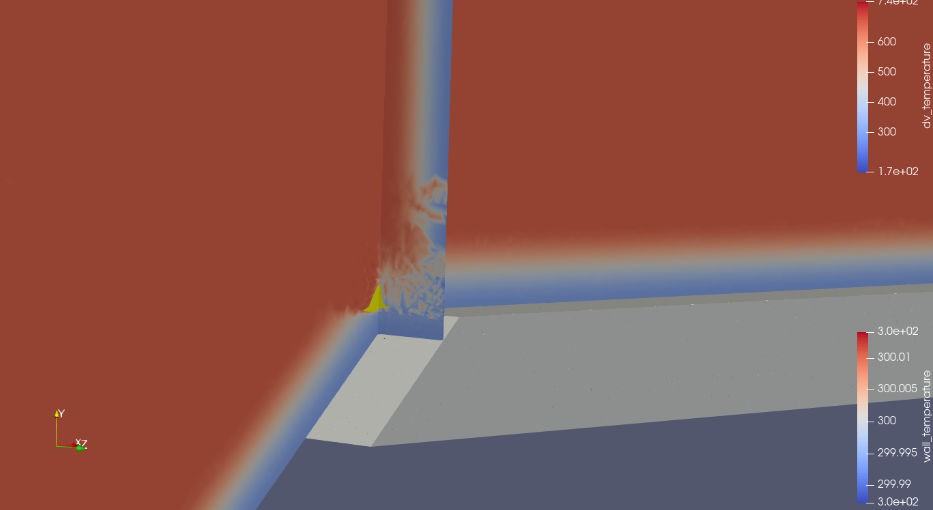
\includegraphics[width=.45\textwidth]{figures/hot_edge.png}
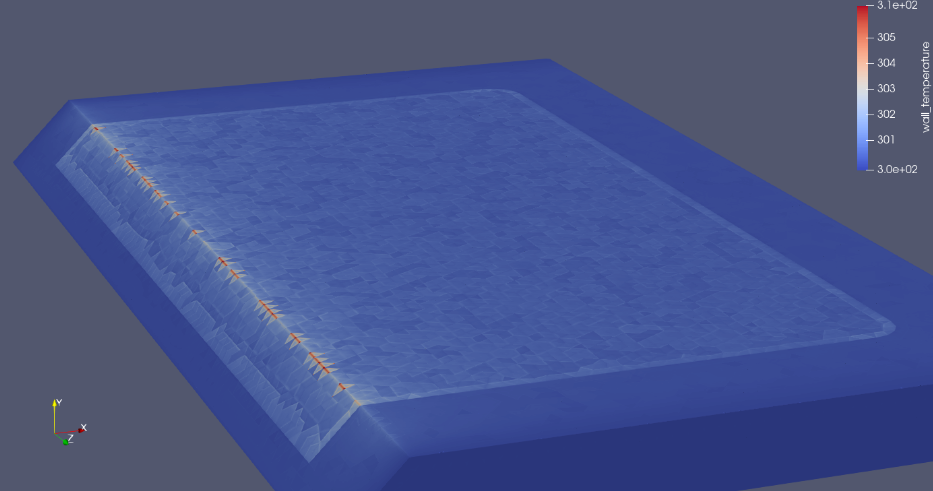
\includegraphics[width=.48\textwidth]{figures/3d_yellow_cells.png}
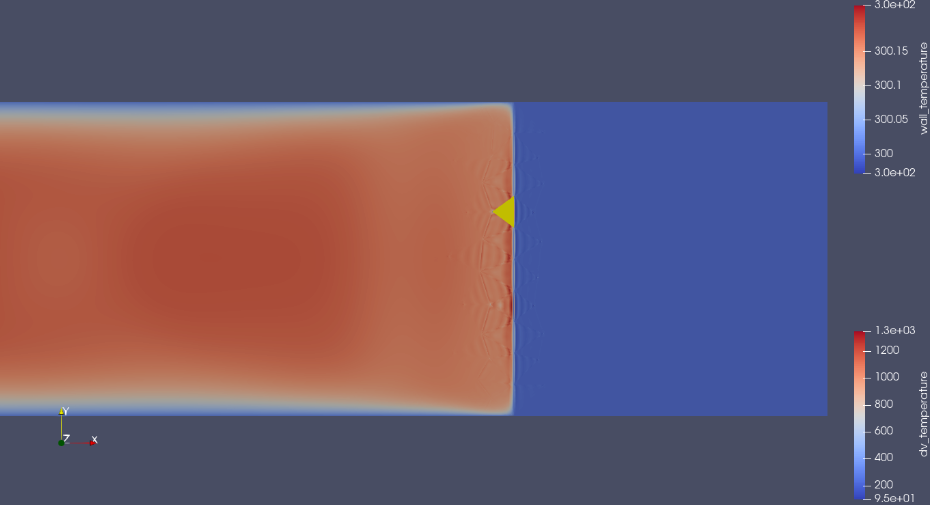
\includegraphics[width=.48\textwidth]{figures/2d_yellow_cells.png}
\end{multicols}
\end{frame}

\begin{frame}\frametitle{Path to Y3 Prediction}
\begin{multicols}{2}
\begin{itemize}
\item Some pain points
  \begin{itemize}
  \item Transfinite or ultra fine mesh to stabilize fluid boundary
    % \begin{itemize}
    % \item Increases complexity of meshing by a lot
    % \item Increases number of elements
    % \item Hex support desired, might help
    % \end{itemize}
  \item Lack confidence in correctness of model implementation
    % \begin{itemize}
    % \item Problem with numerics, or defect?
    % \item More extensive testing!
    % \item More experience/intuition about the numerics
    % \item ESDG?, FV?
    % \end{itemize}
  \item Small problem performance is a drag
    % \begin{itemize}
    % \item 20m compile (this is fine, not fine)
    % \item DAG splat elim, faster compile
    % \end{itemize}
  \item Makes lots of big files
    % \begin{itemize}
    % \item PARSL
    % \item Viz Driver
    % \end{itemize}
  \item Development and testing viscosity
  \item Long queues on available platforms
  \item Cannot change size of run to adapt to resources
  \end{itemize}
\end{itemize}
\end{multicols}
\end{frame}


\begin{frame}\frametitle{Near-term Development Outlook}
\begin{multicols}{2}
\begin{itemize}
\item Now
  \begin{itemize}
  \item Understanding performance (why is it hard?)
    \begin{itemize}
    \item Code $\leftrightarrow$ Kernel \prj{\tiny}{M.~Diener}
    \item Performance model
    \item Kernel rooflines \prj{\tiny}{Nick Christensen}
    \item Feature-specific
    \end{itemize}
  \item Evaluate Tioga
  \item Boundary verif (MMS)
  \item PARSL for testing \prj{\tiny}{D.~Friedel}
  \end{itemize}
\end{itemize}
\columnbreak
\begin{itemize}
\item For prediction: (4mo horizon)
  \begin{itemize}
  \item Radiation \& phenolics \prj{\tiny}{T.~Ricciardi, M.~Smith}
  \item \sout{DAG splat} \prj{\tiny}{Kaushik Kulkarni}
  \item Mechanism parameterization for UQ
  \item PARSL for UQ \prj{\tiny}{D.~Friedel}
  \item Stabilizing prediction runs \prj{\tiny}{M.~Anderson}
    \begin{itemize}
    \item ESDG \prj{\tiny}{Zirui Wang}
    \item Mixed-order
    \item Quad/Hex support \prj{\tiny}{Addison Alvey-Blanco}
    \item Curvlinear elements
    \end{itemize}
  \end{itemize}
\end{itemize}
\end{multicols}
\end{frame}

\begin{frame}\frametitle{Nice to have any time}
\begin{multicols}{2}
\begin{itemize}
\item Reducing prediction pain (important):
  \begin{itemize}
  \item Reduce technical debt (merges)
  \item Driver unification
  \item Help with mesh generation
  \item Visualization driver
  \item PARSL for queue management
  \item M-to-N restart
  \end{itemize}
\item Potentially high-impact performance improvements
  \begin{itemize}
  \item Kernel Autotuning \prj{\tiny}{Nick Christensen}
  \item Node-aware communication \prj{\tiny}{Shelby Lockhart}
  \item DAG/compile time improvements \prj{\tiny}{Kaushik Kulkarni, M.~Diener}
  \item Instrumentation (Mem \& Tags) \prj{\tiny}{Kaushik Kulkarni, M.~Diener}
  \end{itemize}
\item Future sims
  \begin{itemize}
  \item Mesh motion (interface regression)
  \item Wall degradation
  \item Turbulence modeling
  \end{itemize}
\end{itemize}
\end{multicols}
\end{frame}

% CURRENT STATUS OF PERFORMANCE - NEXT TO LAST

%\begin{frame}\frametitle{What is next?}
%\begin{itemize}
%\item Parallel performance is close to prediction, now what?
%%\item Automated performance testing
%%\item Exercise the prediction capability at scale ahead of the science runs
%\item Need to understand our single GPU performance (overall and components)
%\item Flop counting lazy is challenging- No code-to-kernel correspondence is challenging
%\item Tools are in development
%\begin{itemize}
%\item Tools/procedures for understanding kernel flops \prj{\tiny}{Nick Christensen}
%\item Communication analysis and modeling \prj{\tiny}{Shelby Lockhart}
%\item Analysis and profiling tools and development (\prj{\tiny}{Kaushik Kulkarni, M.~Diener}
%\end{itemize}
%\item A performance model is needed - at least for a simple case
%\end{itemize}
%  \begin{tikzpicture}[remember picture, overlay]
%    \fill <2> [fill=white, opacity=0.7] (current page.south west) + (0.5,0.5) rectangle (12.5, 7.8);
%    \node <2> [inner sep=0pt] at (current page.center) {
%      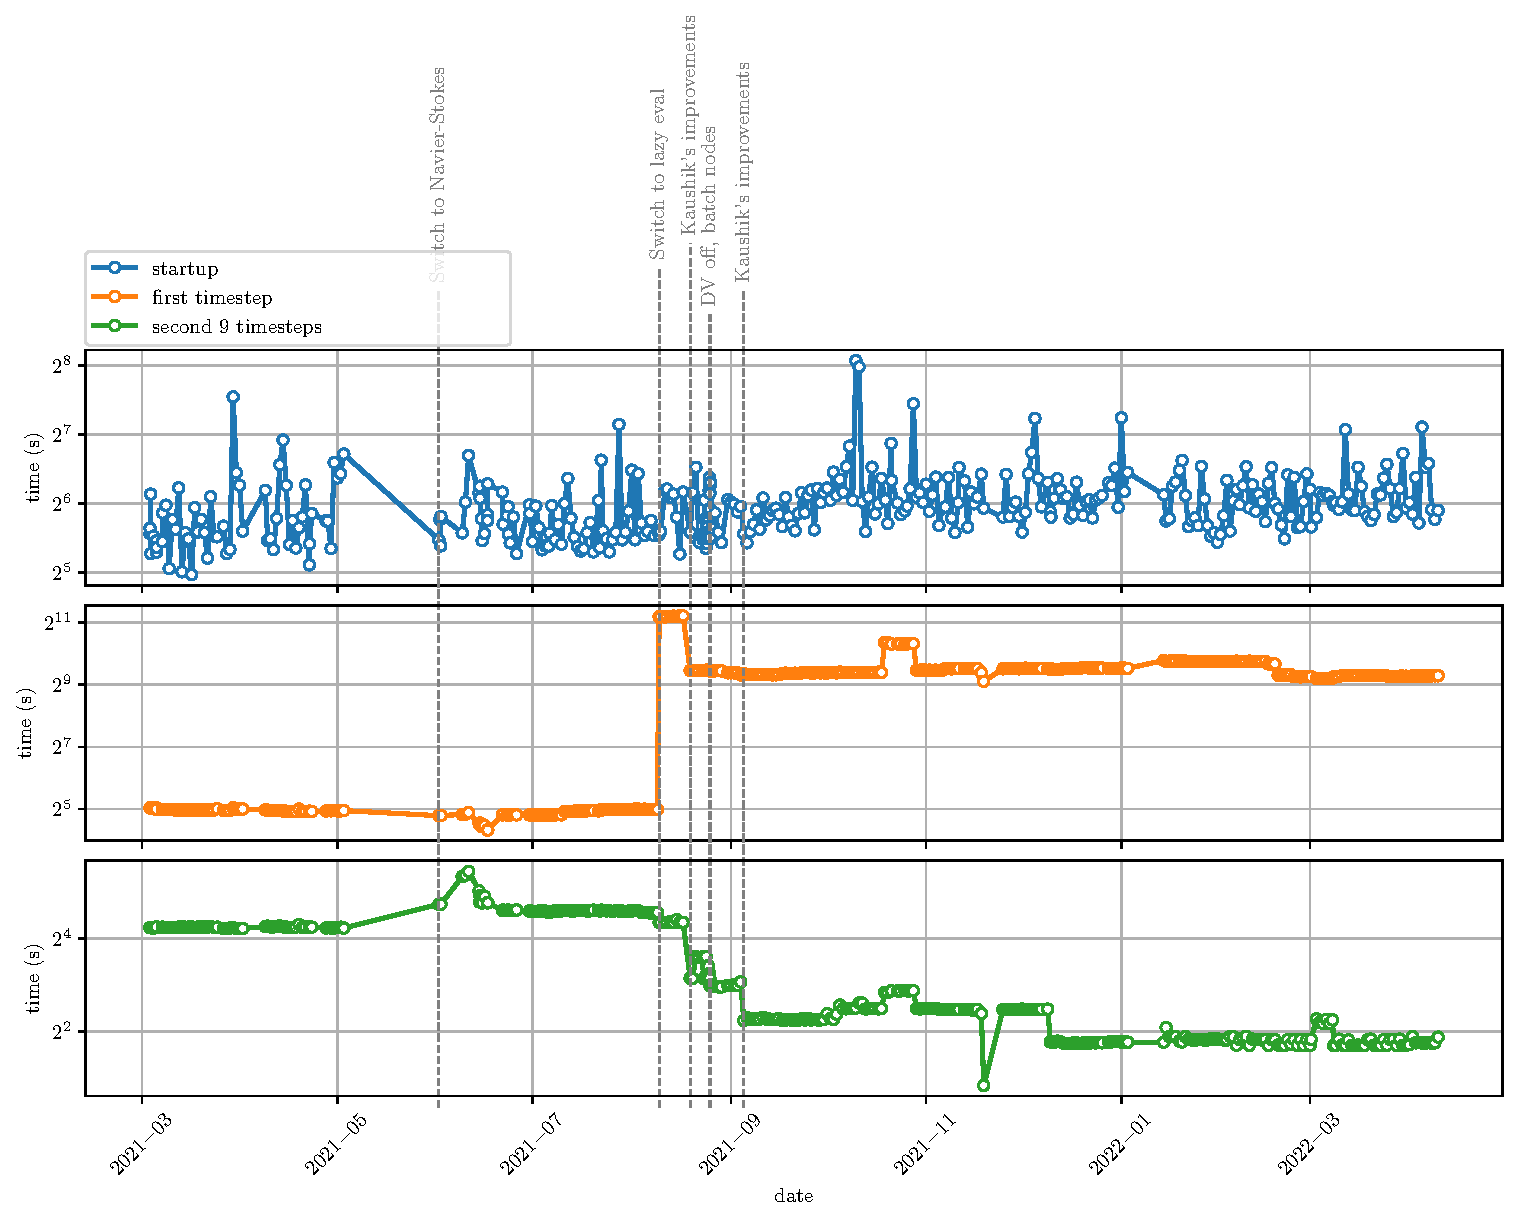
\includegraphics[width=.6\textwidth]{figures/mtc2/nozzle-lazy-full.pdf}
%    };
%  \end{tikzpicture}
%\end{frame}
